\documentclass[preprint,12pt,authoryear]{elsarticle}

% Advances in Space Research -- Elsevier elsarticle preprint workflow.
% Compile on Overleaf or locally with: pdflatex -> bibtex -> pdflatex -> pdflatex

\usepackage[T1]{fontenc}
\usepackage[utf8]{inputenc}
\usepackage{amsmath,amssymb}
\usepackage{booktabs,tabularx,multirow}
\usepackage{graphicx}
\usepackage{enumitem}
\usepackage{microtype}
\usepackage{xurl}
\usepackage[hidelinks]{hyperref}
\emergencystretch=3em
\raggedbottom
\graphicspath{{figures/}}

\journal{Advances in Space Research}
\biboptions{authoryear,round}

\begin{document}

\begin{frontmatter}

\title{Building and evaluating a cross-hazard machine-learning approach to unified lunar forecasting}

\author[aff1]{Luka Takki\corref{cor1}}
\cortext[cor1]{Corresponding author}
\ead{lukatakki123@gmail.com}
\address[aff1]{Affiliation and full postal address required before submission}

\begin{abstract}
LIPAS (Lunar Impact and Predictive Analysis System) is a hybrid forecasting and decision-support platform that combines machine learning with physics-based models to characterize lunar environmental conditions, including temperature, radiation, dust activity, micrometeorite impacts, solar activity, and moonquakes. By unifying NASA and NOAA space-weather products with OMNI telemetry and historical lunar archives, LIPAS produces forecasts through a temporal long short-term memory network constrained by physics-based baselines and presents them in an interactive web dashboard for arbitrary lunar locations.
This study documents the hybrid development process, evaluates operational usability in simulated mission scenarios, and compares locked-model hybrid predictions with replicated public NASA/NOAA-style baselines. Two 14-day windows at three sites show modest solar-activity gains (Window~A RMSE 4.10 versus 4.66; Window~B 4.99 versus 5.99), while radiation does not beat the replica (Window~A 0.119 versus 0.102; quiet dayside Window~B 0.0188 versus 0.00266). Temperature, moonquakes, and dust remain physics ties by design; micrometeorite contrast is limited to a shower-timing term and is circular under blend weight~0. The results support LIPAS as consultative decision support alongside agency products and identify radiation validation, surface measurements, and further hybrid tuning as required next steps.
\end{abstract}

\begin{keyword}
lunar environment \sep space weather \sep hybrid forecasting \sep machine learning \sep long short-term memory \sep mission decision support
\end{keyword}

\end{frontmatter}

\section{Introduction}
\label{sec:intro}

Renewed lunar exploration plans increase the need for readable environmental information for temperature, radiation, dust, micrometeorites, solar activity, and moonquakes \citep{nasa2020artemis}. Specialized models already exist for many of these hazards, but they usually operate as separate tools. LIPAS was built to join public data and hybrid forecasts in one decision-support interface rather than to replace flight-qualified agency systems.

This study asks three questions:
\begin{enumerate}[leftmargin=*,itemsep=0.2em]
\item[\textbf{RQ1}] Can a hybrid lunar forecasting system usefully combine machine learning and physics?
\item[\textbf{RQ2}] Does a unified multi-hazard interface improve operational usability relative to separate products?
\item[\textbf{RQ3}] Does the locked hybrid improve accuracy against selected replicated public baselines?
\end{enumerate}

Because continuous co-located surface truth is not available for every hazard, evaluation uses archived measurements, engineering-model exports, and physics or catalog proxies. That limit is carried through the results and conclusion.

\section{Results}
\label{sec:results}

\subsection{Prototype study and why early wins were large}
\label{sec:prototype}

The first quantitative pass ran in the client-side V1 stack against relatively weak replicas of Diviner-class temperature, radiation, dust, meteor, solar, and seismic products. Under that setup the mean skill across hazards favored LIPAS (Fig.~\ref{fig:proto}). Those early wins are not evidence that the locked hybrid beats mature agency models.

Three design choices drove the spread. First, the client V1 model and scoring path differ from the locked train-2 blend in Eq.~\eqref{eq:blend}. Second, several replica baselines were thin proxies rather than full operational models, so the comparison favored the integrated client. Third, some hazard scores used circular or proxy targets, which inflate apparent skill without independent surface truth. The prototype is therefore treated as an engineering checkpoint only. The locked windows below replace it for accuracy claims.

\begin{figure}[t]
\centering
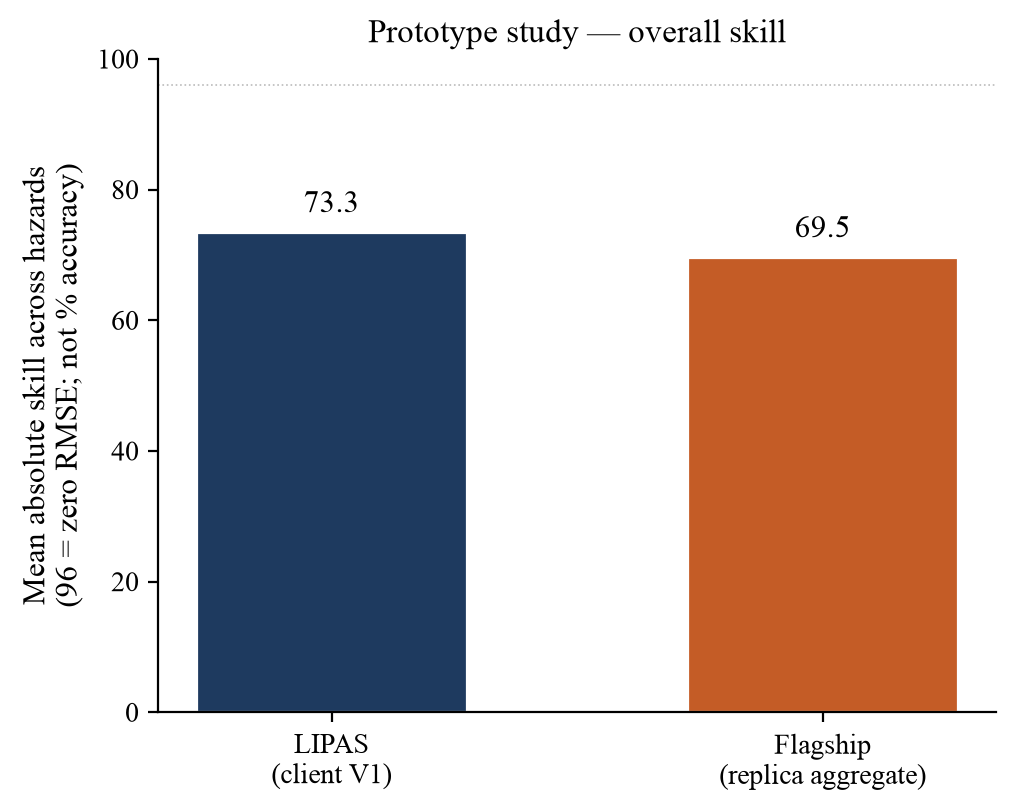
\includegraphics[width=0.72\linewidth]{fig_prototype_lipas_vs_flagship.png}
\caption{Prototype study mean skill: LIPAS (client V1) versus a single flagship-replica aggregate. Two bars only, same within-hazard skill definition as Windows~A and~B. The early lead reflects weak replicas and a different model/scoring path, not the locked train-2 result.}
\label{fig:proto}
\end{figure}

\subsection{LIPAS versus Diviner-class temperature (prototype path)}
\label{sec:diviner}

Figure~\ref{fig:diviner} shows an early daytime temperature comparison at $(0^\circ\mathrm{N},\ 0^\circ\mathrm{E})$ before temperature was locked to the physics path. The early client overshoots the Diviner-class reference and the observed proxy near peak heating. That failure is part of why the locked blend sets temperature weight to zero and why Windows~A and~B report temperature as a physics tie rather than an ML win. The figure belongs to the prototype evaluation era. After this checkpoint the paper moves to the locked studies.

\begin{figure}[t]
\centering
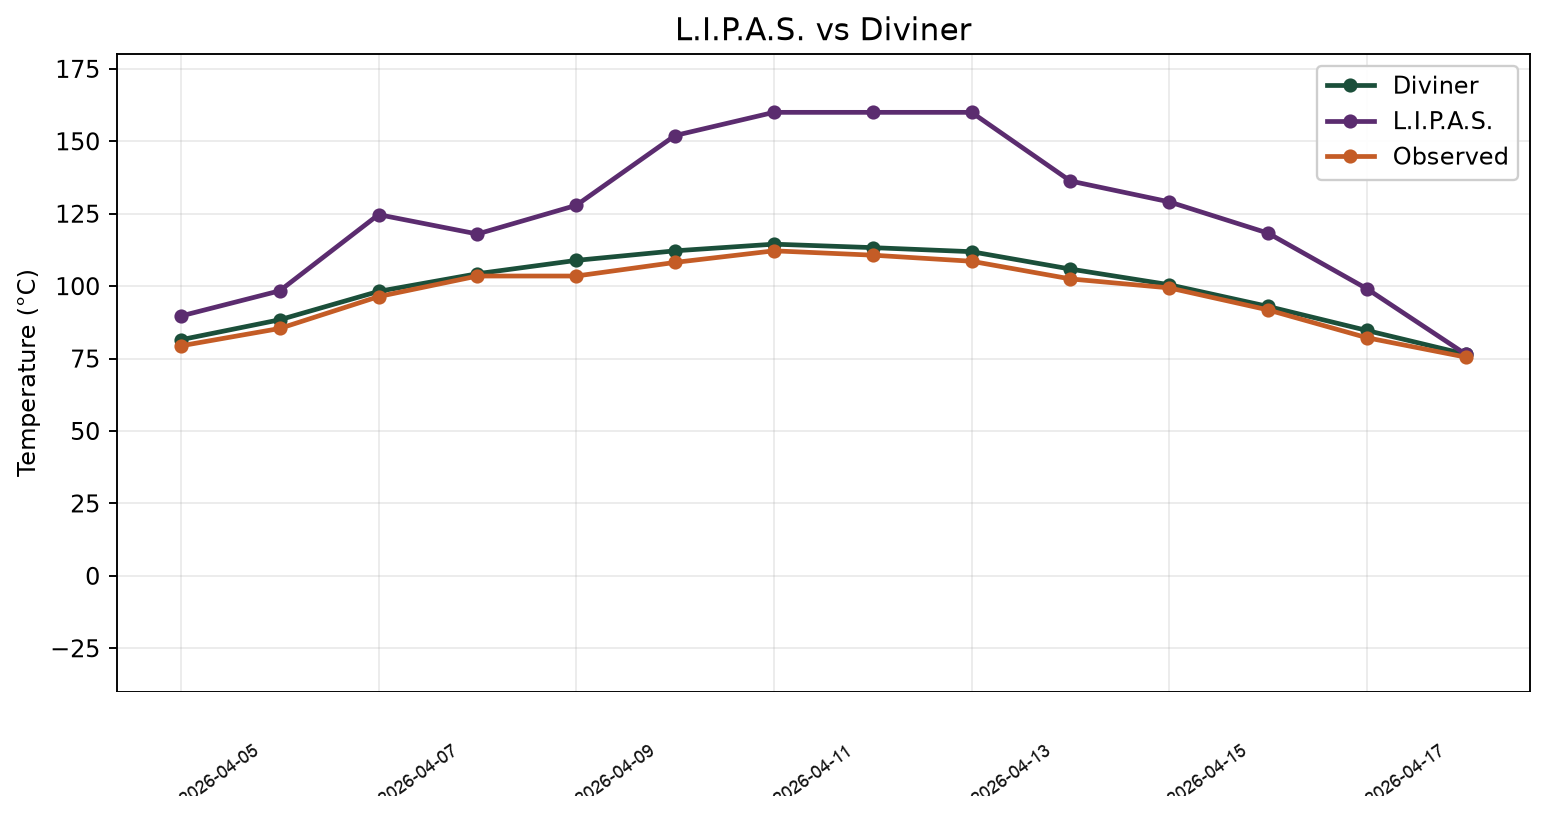
\includegraphics[width=0.92\linewidth]{fig_lipas_vs_diviner.png}
\caption{LIPAS versus Diviner-class temperature reference on the prototype daytime path at $0^\circ\mathrm{N}$, $0^\circ\mathrm{E}$. Early client temperature overshoots the reference near peak heating. Prototype-era figure; locked windows use physics-led temperature under blend weight zero.}
\label{fig:diviner}
\end{figure}

\noindent\textit{Reading Fig.~\ref{fig:diviner} for the prototype study.} The temperature channel did not ``win'' in this early plot. Combined with weak replicas on other channels, that mix is exactly why a single mean-skill bar can still look favorable in Fig.~\ref{fig:proto} while individual physics channels remain untrustworthy. The later locked studies therefore emphasize solar and radiation RMSE, where the replica comparison is more informative, and treat temperature as a shared physics path.

\subsection{Locked Window A (night-dominant)}
\label{sec:windowA}

Window~A uses the locked blend. Solar activity improves relative to the replica (RMSE 4.10 versus 4.66). Radiation does not: night-dominant RMSE is 0.119 for LIPAS versus 0.102 for the replica. Temperature, moonquakes, and dust remain physics ties. Micrometeorite skill is circular under blend weight zero and is not treated as an independent win.

\begin{figure}[t]
\centering
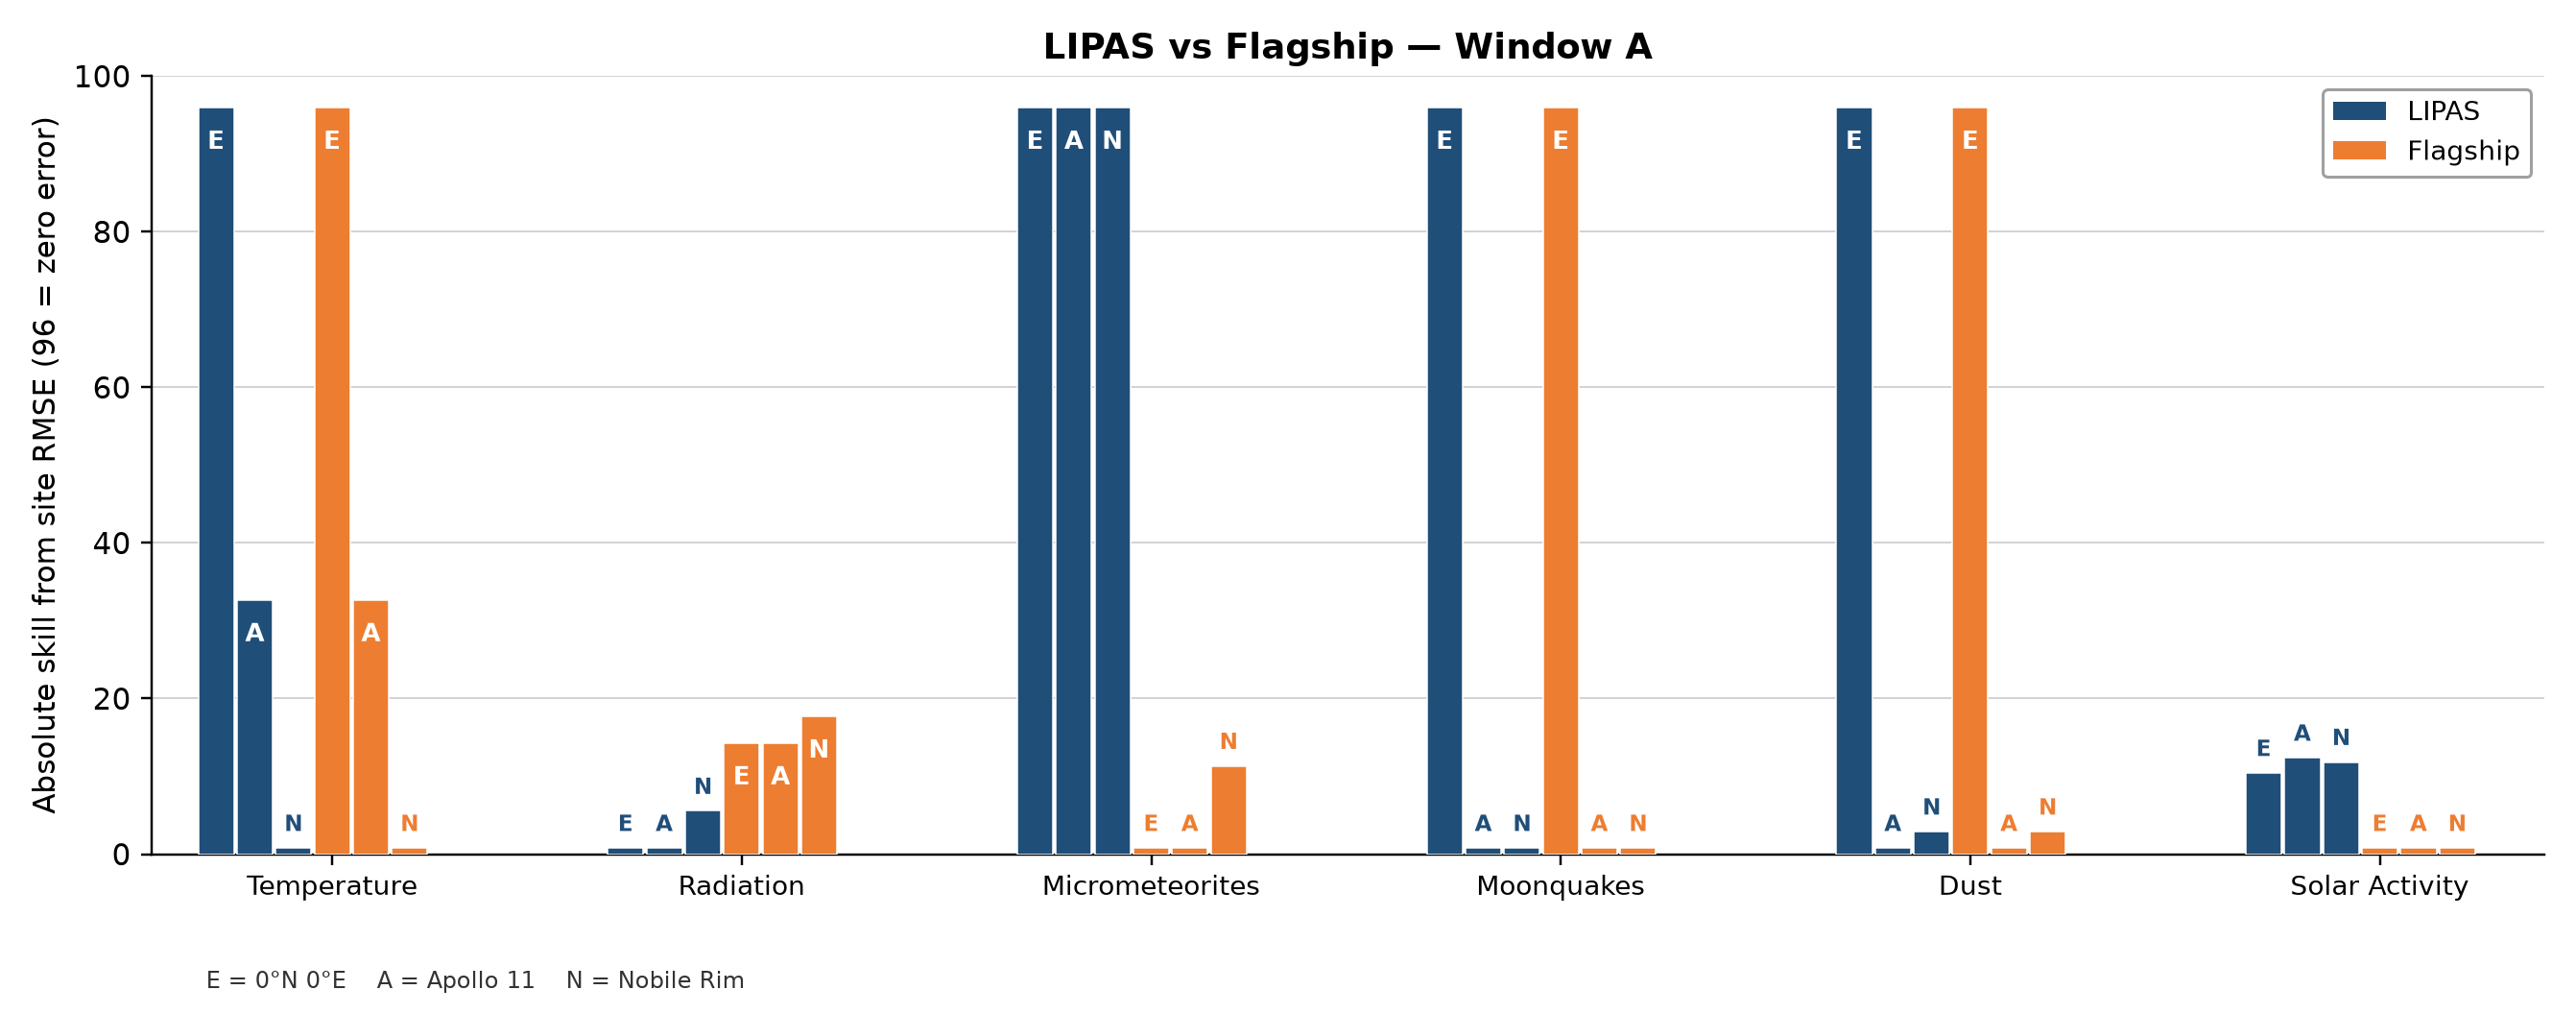
\includegraphics[width=0.95\linewidth]{fig_windowA_skill.png}
\caption{Window~A locked skill by hazard and site. Within-hazard skill only; no cross-hazard height equalization. Location key: E = $0^\circ\mathrm{N}$, $0^\circ\mathrm{E}$; A = Apollo~11; N = Nobile Rim.}
\label{fig:wa}
\end{figure}

\subsection{Locked Window B (dayside quiet)}
\label{sec:windowB}

Window~B again shows a solar gain (RMSE 4.99 versus 5.99) while radiation remains worse than the replica under quiet dayside conditions (0.0188 versus 0.00266). Physics ties and circular micrometeorite scoring match Window~A.

\begin{figure}[t]
\centering
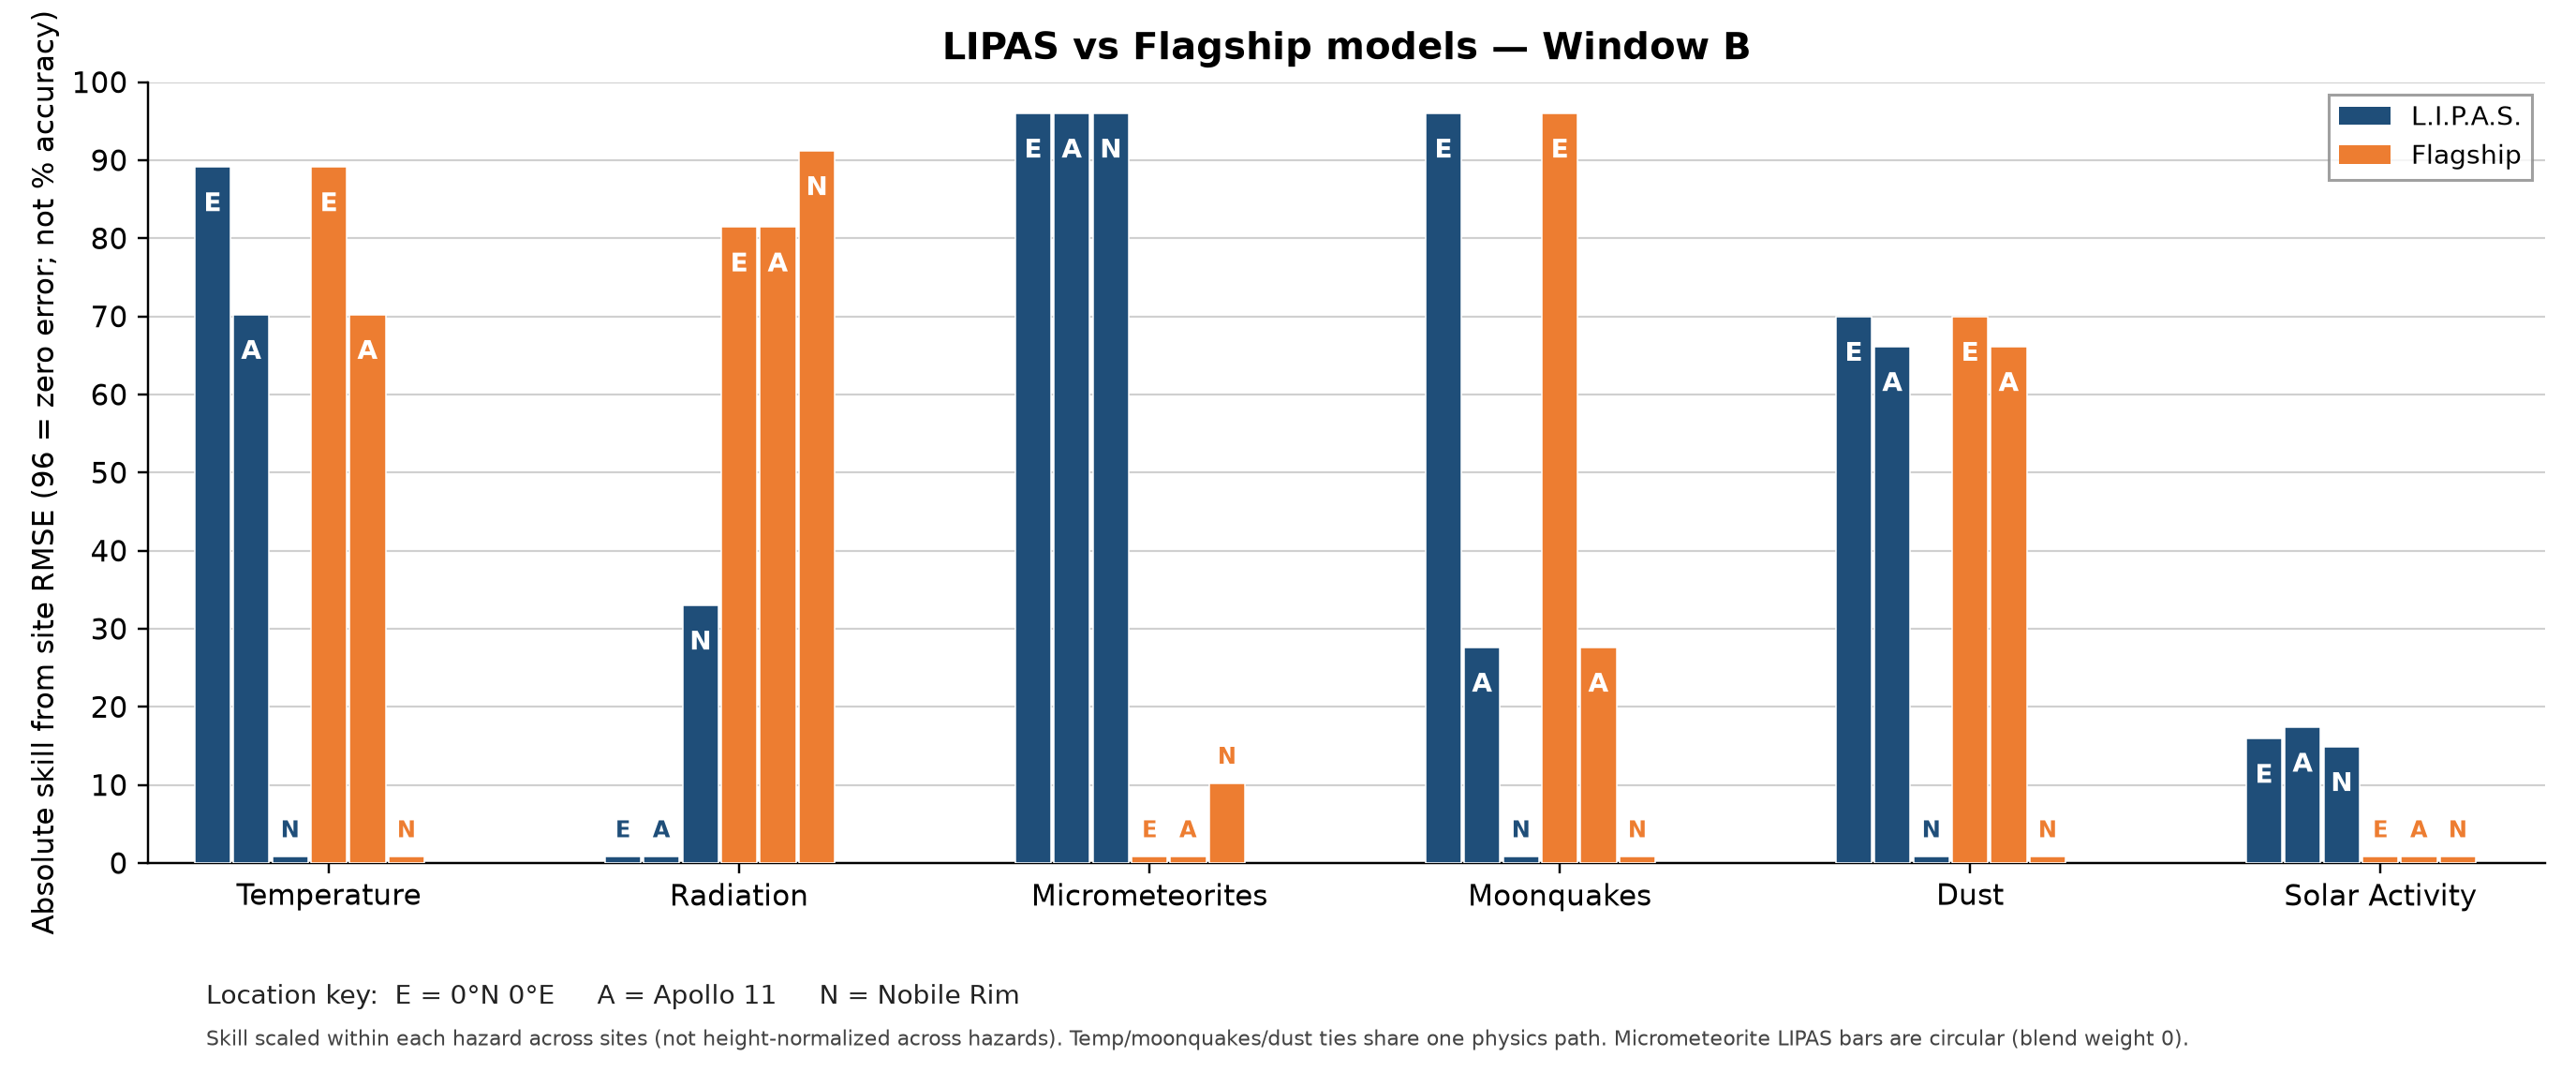
\includegraphics[width=0.95\linewidth]{fig_windowB_skill.png}
\caption{Window~B locked skill by hazard and site. Same blend and replica stack as Window~A. Location key as in Fig.~\ref{fig:wa}.}
\label{fig:wb}
\end{figure}

\subsection{Qualitative comparison}
\label{sec:qual}

A structured qualitative framework scores nine criteria (coverage, fusion, forecasting, spatial reach, real-time operations, robustness, validation, usability, openness) against DONKI, Diviner, LDEX, Apollo PSE, MEM~3, and GOES-18 (full rubric and references in Appendix~B). LIPAS ranks high on multi-hazard coverage, fusion, and dashboard usability: one interface exposes six hazards and selectable lunar coordinates. Validation and robustness are only moderate because continuous co-located surface truth is missing for several hazards and because many scores rely on proxies. Specialized agency products invert that pattern: high validation inside one domain, low multi-hazard coverage.

For the research questions this means: RQ2 is supported on usability and coverage; RQ3 is only partly supported and must rest on the locked windows, not on the prototype bars; RQ1 is supported as a working hybrid architecture but not as a claim of uniform accuracy gains. Deeper interpretation of trade-offs is taken up in Section~\ref{sec:discussion}.

\subsection{Mission simulation}
\label{sec:mission}

A short mission timeline overlays caution and no-go markers for planning context (Fig.~\ref{fig:mission}). Legend markers use red for all compared paths so the timeline reads cleanly in print. This study is operational illustration, not a substitute for the locked RMSE tables.

\begin{figure}[t]
\centering
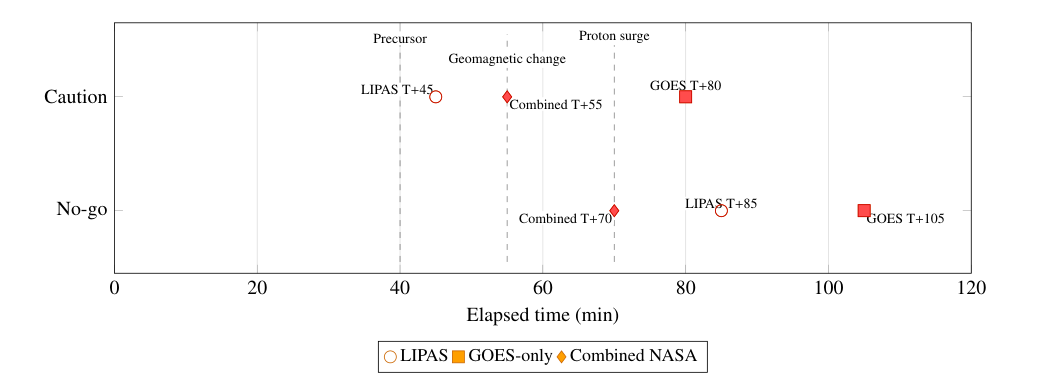
\includegraphics[width=0.95\linewidth]{fig_mission_timeline.png}
\caption{Mission simulation timeline with caution and no-go markers. Legend uses red markers for LIPAS, GOES-only, and Combined NASA paths. Operational context only.}
\label{fig:mission}
\end{figure}

\subsection{Ablation}
\label{sec:ablation}

Hazard-weight ablation shows that nonzero machine-learning weight on solar activity and radiation changes residuals as expected under Eq.~\eqref{eq:blend}, while zero-weight hazards stay on their physics or proxy paths. Ablation supports sensitivity interpretation; it does not create new locked wins.
\section{Discussion}
\label{sec:discussion}

\subsection{Cross-experiment reading}
\label{sec:rq}

\paragraph{RQ1 (development).}
A channel-specific hybrid approach was more appropriate than applying machine learning uniformly. Physics-tied channels stay on shared paths; learned corrections help where drivers add information, especially solar activity, not radiation.

\paragraph{RQ2 (usability).}
The unified dashboard improved how information is presented for planning, but this study did not show that LIPAS is safer than existing agency pathways.

\paragraph{RQ3 (accuracy).}
Solar RMSE is lower in both windows. Radiation is not: Window~A hybrid 0.119 versus replica 0.102; quiet Window~B 0.0188 versus 0.00266. Temperature, moonquakes, and dust stay physics-aligned. Micrometeorite skill reflects the shower-timing term only.

Mission simulation: LIPAS issued caution earlier than the GOES-only path by using upstream drivers; the combined NASA path still produced the earlier hard no-go. Treat LIPAS as consultative decision support alongside agency products.

Ablation: setting solar input to its Window~A mean lowered solar RMSE and raised radiation RMSE in that quiet interval. This is sensitivity, not evidence that live solar data are generally harmful.

\subsection{Why radiation is worse, and why Window~B looks worse relatively}
\label{sec:why-rad}

The absence of improvement in temperature, moonquakes, and dust is a consequence of design rather than necessarily a weakness: those channels were deliberately physics-led. The clearest evidence for additional learned information came from the modest solar-activity reductions rather than any radiation win over the replica.

Window contrast matters. Window~A is night-dominant with higher absolute radiation labels; the hybrid still trails the replica, but absolute RMSEs are of similar order (0.119 versus 0.102). Window~B is quiet dayside: absolute doses collapse, the replica stays close to the quiet path, and the small radiation blend ($0.05$) plus low-biased ML corrections inflate relative error (0.0188 versus 0.00266). Hybrid beats raw ML-only radiation ($\sim$0.068 in Window~B) but remains worse than physics/replica. This is a quiet-regime radiation-channel limit, not evidence that LIPAS is broken overall---but it must be reported honestly and improved before operational claims.

What could be made better: denser OMNI/DONKI/SWPC sampling across active intervals, calibrated uncertainty on the radiation blend, storm-period holdouts, and eventual replacement of proxy labels with Artemis-era surface measurements.

\subsection{Limitations}
\label{sec:limits}

Quantitative targets use public observations, physical formulations, catalogs, and proxies rather than continuous co-located lunar-surface truth. Agency comparisons are independent public-method reconstructions (except the available MEM~3 engineering-model export), not certified operational NASA/NOAA software. Combining physics and machine learning is not itself new \citep{karpatne2017,willard2022,camporeale2019}; LIPAS's contribution is hazard-specific weighting and unified decision support under incomplete observations.

\section{Conclusion}
\label{sec:conclusion}

This research shows how machine learning can be integrated into a unified, physics-based lunar-forecasting system while retaining the physical foundations of established environmental models. The development process answered the first research question by showing that a hazard-specific hybrid approach was appropriate for the current model, rather than applying machine learning uniformly across all hazards. The operational evaluation answered the second by showing that integrating hazards and data sources can improve how information is presented during mission planning, but it did not establish that LIPAS is safer than existing approaches. A unified system can also concentrate risk if its data or service fails. LIPAS is best considered alongside current NASA and NOAA systems as a consultative decision-support tool, subject to validation with real mission workflows and measurements.

The quantitative evaluation answered the third selectively. Chronological holdout RMSE was about 4.97 versus about 13.66 for persistence, and solar activity improved modestly in both windows. Radiation did not: hybrid RMSE exceeded the replica in night-dominant Window~A (0.119 versus 0.102) and in quiet dayside Window~B (0.0188 versus 0.00266). Temperature, moonquakes, and dust remained physics ties. Micrometeorite skill is circular under blend weight~0 and remains shower-term descriptive only. These studies therefore teach where the hybrid helps and where it still fails.

The central result is that a carefully constrained hybrid architecture can add predictive capability where machine learning is useful without replacing physics-based methods where they are more appropriate. LIPAS's principal contribution is therefore not the replacement of existing lunar models, but their integration into a single forecasting and decision-support framework.

The findings must be read with those limits in mind: proxy labels, quiet-regime radiation shortfalls, and circular micrometeorite scoring. LIPAS should function alongside NASA and NOAA products as consultative decision support, not as a replacement. The studies show how much remains to develop---radiation under quiet and storm regimes, stronger validation with surface measurements, and clearer operational workflows. This work does not end here; it is a first constrained step that the next iterations must extend.

\section*{Acknowledgements}
The author thanks Marjo Lipponen-Mraz for mentorship and Benjamin Irani-Fey for coding support during the NASA Space Apps Challenge. The author also thanks NASA, NOAA, and other space agencies and research organizations for the public lunar-mission data and space-weather archives that made the project possible, and Polygence research mentor Kyle Kennedy for support in redesigning and re-evaluating the studies, methods, and conclusions.

\section*{CRediT author statement}
\textbf{Luka Takki:} Conceptualization, Methodology, Software, Validation, Formal analysis, Investigation, Data curation, Visualization, Writing --- original draft, and Writing --- review and editing.

\section*{Funding}
This research received no specific grant from funding agencies in the public, commercial, or not-for-profit sectors.

\section*{Declaration of competing interest}
The author declares that there are no known competing financial interests or personal relationships that could have appeared to influence the work reported in this paper.

\section*{Data and code availability}
The evaluation uses public NASA, NOAA, OMNI, Diviner, CRaTER, LADEE/LDEX, Apollo, MEM~3, and meteor-shower sources listed in the references. Code, locked model files, and numerical tables:
\url{https://github.com/Luka-bot-afk/LIPAS}. Daily tables are in \path{papers/appendix_numerical_tables/}. Reported window RMSE values matching Tables~\ref{tab:wa}--\ref{tab:wb} are in \path{papers/appendix_numerical_tables/reported_window_rmse.md}.

\section*{Declaration of generative AI and AI-assisted technologies in the manuscript preparation process}
During the preparation of this work, I used Cursor and Google Gemini to review, and to help modify, selected parts of the code and the manuscript. These tools did not write the paper. I checked every suggested change, made the final edits myself, and take full responsibility for the content of the published article. Their role was limited to review and selective modification of existing material; they were not used to draft or author the manuscript.


\bibliographystyle{elsarticle-harv}
\bibliography{references}

\end{document}
